\documentclass[conference]{IEEEtran}
\IEEEoverridecommandlockouts
\usepackage{cite}
\usepackage{amsmath,amssymb,amsfonts}
\usepackage{algorithmic}
\usepackage{graphicx}
\usepackage{textcomp}
\usepackage{xcolor}
\usepackage{hyperref}
\usepackage{algorithm}
\usepackage{booktabs}
\usepackage{multirow}
\usepackage[font=small,labelfont=bf]{caption}
\def\BibTeX{{\rm B\kern-.05em{\sc i\kern-.025em b}\kern-.08em
    T\kern-.1667em\lower.7ex\hbox{E}\kern-.125emX}}
\begin{document}

\title{\textbf{Near-Optimal Robotic Sorting via Solver Distillation into Cycle-Aware Graph Neural Networks}}

\author{\IEEEauthorblockN{1\textsuperscript{st} Given Name Surname}
\IEEEauthorblockA{\textit{dept. name of organization (of Aff.)} \\
\textit{name of organization (of Aff.)}\\
City, Country \\
email address or ORCID}
\and
\IEEEauthorblockN{2\textsuperscript{nd} Given Name Surname}
\IEEEauthorblockA{\textit{dept. name of organization (of Aff.)} \\
\textit{name of organization (of Aff.)}\\
City, Country \\
email address or ORCID}
\and
\IEEEauthorblockN{3\textsuperscript{rd} Given Name Surname}
\IEEEauthorblockA{\textit{dept. name of organization (of Aff.)} \\
\textit{name of organization (of Aff.)}\\
City, Country \\
email address or ORCID}
}

\maketitle

\begin{abstract}
Integer Linear Programming (ILP) solvers produce provably optimal pick-and-place (PAP) sequences but become intractable beyond ${\sim}30$--$40$ objects, while greedy heuristics scale trivially yet sacrifice 3--5\% in travel cost even when accounting for placement distance, and up to 10--40\% in constrained conveyor settings \cite{han2019pap}. We bridge this gap by \emph{distilling} the decision quality of an ILP solver into a lightweight Graph Neural Network (GNN) policy. The key enabler is a cycle-aware directed graph whose two cost-bearing edges encode the robot-to-object pick leg and object-to-bin place leg, closed by a bin-to-robot feedback edge that routes the robot's post-placement position back into the decision for the next step. Three semantically distinct node types (robot, object, bin) with type-encoded features are processed by a standard Graph Attention Network, capturing structural information discarded by flat sequence-to-sequence neural combinatorial optimisation (NCO) architectures. Trained via curriculum-based imitation learning on ILP-optimal prefixes with greedy fallback, the policy reaches a mean ILP gap of 1.81\% at $N{=}10$ (matching the optimum exactly on the easiest instances), improves 3.23\% over greedy on average at $N{=}40$, and wins on 98\% of 100 held-out scenarios ($p < 10^{-31}$, paired $t$-test). Crucially, it scales to $N{=}200$ objects where ILP is entirely infeasible, extending near-optimal decision-making beyond the reach of the exact solver itself.
\end{abstract}

\begin{IEEEkeywords}
Graph Neural Networks, Solver Distillation, Imitation Learning, Curriculum Learning, Pick-and-Place Sequencing, Robotic Sorting, Combinatorial Optimization.
\end{IEEEkeywords}

%========================================================================
\section{Introduction}
%========================================================================

Pick-and-place (PAP) sequencing is a core planning task in robotic automation: a manipulator must determine the order in which to pick objects from a workspace and deposit them into designated bins so as to minimise total travel time. The problem is NP-hard \cite{chalasani1996}; the $N!$ candidate sequences grow combinatorially, making exhaustive search impractical beyond toy instances. It arises in warehouse bin picking (where order-picking accounts for a substantial share of operational costs \cite{cheng2024drl}), automated waste sorting in material recovery facilities \cite{gundupalli2021sequence, kiyokawa2024challenges}, and robotic kitting in manufacturing.

Current industrial systems default to greedy nearest-neighbour heuristics that run in $O(n^2)$. Even when the heuristic accounts for the full pick-and-place cycle cost (choosing the object that minimises the sum of pick \emph{and} placement distance), it remains myopic: each decision optimises a single step without considering how the robot's resulting position affects downstream picks. This short-horizon reasoning cascades through the sequence, accumulating suboptimality. Exact ILP solvers guarantee optimality but scale exponentially; beyond $N \approx 30$--$40$ objects, solve times exceed real-time budgets. This leaves a critical capability gap.

We propose to close this gap by treating the ILP solver as a \emph{teacher} and a GNN as a \emph{student}: the exact solver produces provably optimal sequence prefixes offline, and the GNN learns to reproduce that reasoning at bounded, predictable inference cost. At deployment, the student runs alone, delivering ILP-quality sequences in milliseconds and, crucially, generalising to problem sizes ($N{=}100$, $N{=}200$) where the teacher is entirely intractable. The scalability story is the central contribution: we extend the reach of exact combinatorial optimisation beyond the solver's own computational limits.

Two structural insights enable this distillation. First, PAP is \emph{not} symmetric TSP: the cost of picking object $i$ followed by object $j$ depends on which bin $i$ was deposited in, since the robot's position after placing $i$ is $b_{\tau(i)}$, not $o_i$. This asymmetry is precisely why Pointer Networks \cite{vinyals2015pointer} and attention-based models \cite{kool2019attention}, which embed all nodes as homogeneous 2D coordinates, require structural modification to handle PAP. Second, the pick-and-place action has an inherent \emph{cyclic} structure (robot$\to$object$\to$bin$\to$robot) that is naturally represented as a directed graph but is invisible to flat sequence encoders.

We make the following contributions:
\begin{enumerate}
    \item A \textbf{cycle-aware graph formulation} for PAP sequencing that explicitly models the pick-place cycle with three semantically distinct node types (robot, object, bin) connected by directed edges encoding pick, place, and feedback legs. Type information is encoded in node features and processed by a standard GAT, unlike prior flat NCO formulations that discard this relational structure.
    \item A \textbf{cycle-aware GNN architecture} (2-layer GAT on the cyclic star topology) that reasons jointly over pick and placement costs by propagating information along the causal path of each candidate action.
    \item A \textbf{multi-fidelity imitation learning framework} that augments ILP-optimal prefix supervision with greedy-heuristic fallback under a curriculum schedule. The contribution is not quality-improving (ILP-only supervision achieves a comparable per-scenario gap; see Table~\ref{tab:ablations}) but \emph{coverage-enabling}: it allows the curriculum to continue training when ILP prefixes are absent at large $N$, and reduces total training wall-clock time by eliminating the need to wait for additional ILP solves before each curriculum stage.
    \item \textbf{Empirical demonstration} of near-optimal performance: 1.81\% mean ILP gap at $N{=}10$ (with exact matches on the easiest instances), 98\% win-rate vs.\ greedy at $N{=}40$ on 100 held-out scenarios, and scalability to $N{=}200$ well beyond ILP limits.
    \item An \textbf{analysis of planning horizon} investigating where in the sequence the GNN's cost advantage accumulates, suggesting that greedy myopia concentrates in late-sequence steps.
\end{enumerate}

The remainder of this paper is organised as follows. Section~\ref{sec:lit} reviews related work. Section~\ref{sec:methods} presents the problem formulation, graph representation, architecture, and training. Section~\ref{sec:data} describes the dataset. Section~\ref{sec:results} reports results, ablations, and analysis. Section~\ref{sec:conclusion} concludes.

%========================================================================
\section{Literature Review}\label{sec:lit}
%========================================================================

\subsection{PAP Sequencing and Its Relation to TSP}

PAP shares combinatorial structure with TSP \cite{dantzig1954}, but is structurally richer: TSP involves a single homogeneous node type and symmetric costs, while PAP has three entity types (robot, object, bin) and asymmetric cycle costs. Collapsing PAP to TSP by treating each object as a city discards the bin assignment and falsely assumes the cost of visiting object $i$ then $j$ is independent of which bin $i$ was deposited in.

\subsection{Greedy Methods and Their Limits}

The nearest-neighbour heuristic \cite{rosenkrantz1977} runs in $O(n^2)$ with a worst-case $\Theta(\log n)$ approximation ratio. In PAP, two natural greedy variants exist: \emph{Nearest Neighbor} (NN), which selects the object closest to the robot (minimising only the pick leg $\lVert r_t - o_i \rVert$), and \emph{Nearest Cycle} (NC), which selects the object minimising the full pick-and-place step cost $\lVert r_t - o_i \rVert + \lVert o_i - b_{\tau(i)} \rVert$. NC is strictly stronger than NN because it accounts for the placement leg; however, it remains myopic: it cannot reason about how the robot's post-placement position affects the cost of future picks, leading to cascading suboptimality. Han, Feng, and Yu \cite{han2019pap} formally prove greedy variants are suboptimal in conveyor PAP and demonstrate 10--40\% efficiency loss versus dynamic programming on SCARA and Delta robots.

\textbf{Important:} Throughout this paper, our greedy baseline refers to the stronger NC variant. All reported greedy costs, win-rates, and gap percentages are computed against NC, not NN. This makes our comparisons conservative: improvements over NC are harder to achieve than improvements over NN.

\subsection{Sequence-to-Sequence NCO}

Vinyals et al.\ \cite{vinyals2015pointer} introduced Pointer Networks for combinatorial sequencing via attention over the input set. Kool et al.\ \cite{kool2019attention} replaced the LSTM encoder with a Transformer, achieving state-of-the-art TSP results via REINFORCE. Both encode each node as a 2D coordinate with no mechanism for typed edges or distinct node roles, making PAP application require ad-hoc preprocessing that discards relational structure.

\subsection{Symmetry-Exploiting RL}

POMO \cite{kwon2020pomo} and Sym-NCO \cite{kim2022symnco} exploit TSP cost symmetries (start-node invariance, rotation/reflection). Neither assumption holds in PAP: the robot home is a fixed asymmetric anchor, bin locations are type-specific, and conveyors introduce directional bias.

\subsection{Improvement-Based RL}

Costa et al.\ \cite{costa2020learning2opt} trained an RL agent for 2-opt local search. In PAP, a swap involves two full pick-place cycles whose cost depends on bin assignment, breaking the symmetric 2-opt operator definition.

\subsection{Constrained Routing Transformers}

Xiong et al.\ \cite{xiong2025ropt} proposed RoPT for last-mile delivery with time-window constraints, using learned decoder masks analogous to our logit masking. However, all nodes share identical feature structures; semantically distinct node types are not addressed.

\subsection{Graph Pointer Networks}

Perera et al.\ \cite{perera2023gpn} combined a GNN encoder with a Pointer Network decoder for TSP. This is the closest prior architecture to ours, but operates on a homogeneous graph of 2D cities. Our advance is the cycle-aware star topology with three semantically distinct node types and directed edges encoding pick-place-feedback cycles.

\subsection{GNNs for Combinatorial Optimisation}

Cappart et al.\ \cite{cappart2023gnnco} argue that GNNs are the natural architecture for CO due to permutation invariance, sparsity awareness, and flexibility for richer node types and constraints. Chung et al.\ \cite{chung2025ncosurvey} identify industrial sequencing as an underexplored NCO domain, with PAP requiring structural modification beyond standard TSP formulations.

\subsection{Why GNNs Outperform Sequence Models for PAP}

The case has three layers. \textbf{Structural representation:} PAP has three node types and asymmetric edge costs; GNNs encode this naturally while sequence models collapse all entities into one embedding space. \textbf{Permutation invariance:} GNNs are invariant to node ordering by construction; our GAT encoder handles all three types simultaneously. \textbf{Dynamic graph:} As objects are picked, the graph changes; our dynamic edge construction handles this at every step without re-encoding.

%========================================================================
\section{Methods}\label{sec:methods}
%========================================================================

We formulate PAP sequencing as a sequential decision process and train a GNN policy via imitation learning on ILP-optimal prefixes. The pipeline consists of four stages: (1) procedural scenario generation, (2) offline expert annotation via ILP and greedy solvers, (3) curriculum-based imitation learning, and (4) autoregressive inference rollout.

\subsection{Problem Formulation and Cost Model}

We consider a planar PAP task in a $W \times W$ workspace ($W=100$). At each step $t$, the agent selects one remaining object $a_t$ to pick and place into its assigned bin. The robot starts at $r_0 \in \mathbb{R}^2$ and updates its pose to the bin location after each placement. The step cost is:
\begin{equation}
c_t = \lVert r_t - o_{a_t} \rVert_2 + \lVert o_{a_t} - b_{\tau(a_t)} \rVert_2,
\end{equation}
where $o_{a_t}$ is the object position and $b_{\tau(a_t)}$ is the target bin for object type $\tau(\cdot)$. The objective is to minimise total cost $C = \sum_{t=1}^{N} c_t$.

The cost is asymmetric: picking $i$ then $j$ costs differently depending on which bin $i$ was deposited in, since $r_{t+1} = b_{\tau(i)}$. This asymmetry distinguishes PAP from TSP and is the structural reason why TSP-specific methods require modification. For $N$ objects the search space is $N!$; exact methods require $O(2^n \cdot n)$ operations \cite{han2019pap}, limiting them to $N \approx 30$--$40$ within real-time budgets ($<$500~ms).

\subsection{Graph Representation}

We model the state $S_t$ as a directed graph $\mathcal{G}_t = (\mathcal{V}, \mathcal{E})$ with three semantically distinct node types and directed edges encoding the causal structure of pick-and-place actions. Node type information is encoded in the feature vectors rather than through separate message-passing channels.

\subsubsection{Node Types and Features}
The vertex set $\mathcal{V}$ comprises: one robot node, $N$ object nodes, and $M{=}4$ bin nodes. Each node carries a feature vector of dimension $F = 4 + M + 1 = 9$, encoding normalised spatial coordinates, a reference position (target bin for objects), a one-hot type encoding, and a binary availability mask. Full feature vector specifications are provided in Appendix~\ref{app:features}.

\subsubsection{Cyclic Star Topology}\label{sec:topology}
Unlike fully connected graphs used in standard NCO, the proposed topology explicitly encodes the \emph{causal structure} of pick-and-place actions. For each remaining object $i$, we construct three directed edges forming a cycle:

\textbf{Robot $\to$ Object $i$:} Represents the pick-leg, implicitly encoding distance $\lVert r_t - o_i \rVert$.

\textbf{Object $i$ $\to$ Bin $\tau(i)$:} Represents the place-leg, encoding $\lVert o_i - b_{\tau(i)} \rVert$.

\textbf{Bin $\tau(i)$ $\to$ Robot (feedback edge, not a travel leg):} Closes the cycle so that the robot's post-placement position, which becomes its starting position for the next decision, participates in message passing. This edge does \emph{not} correspond to any physical robot motion and contributes no cost term; after placing object $i$, the robot moves directly to the next picked object from the bin location.

This yields a compact \emph{cyclic star graph} (Fig.~\ref{fig:graph_topology}) where each candidate action corresponds to a directed 3-edge cycle. The topology is a structural inductive bias: two layers of message passing propagate information around each full cycle, allowing object node embeddings to encode the complete pick-place cost before scoring.


\begin{figure}[htbp]
\centering
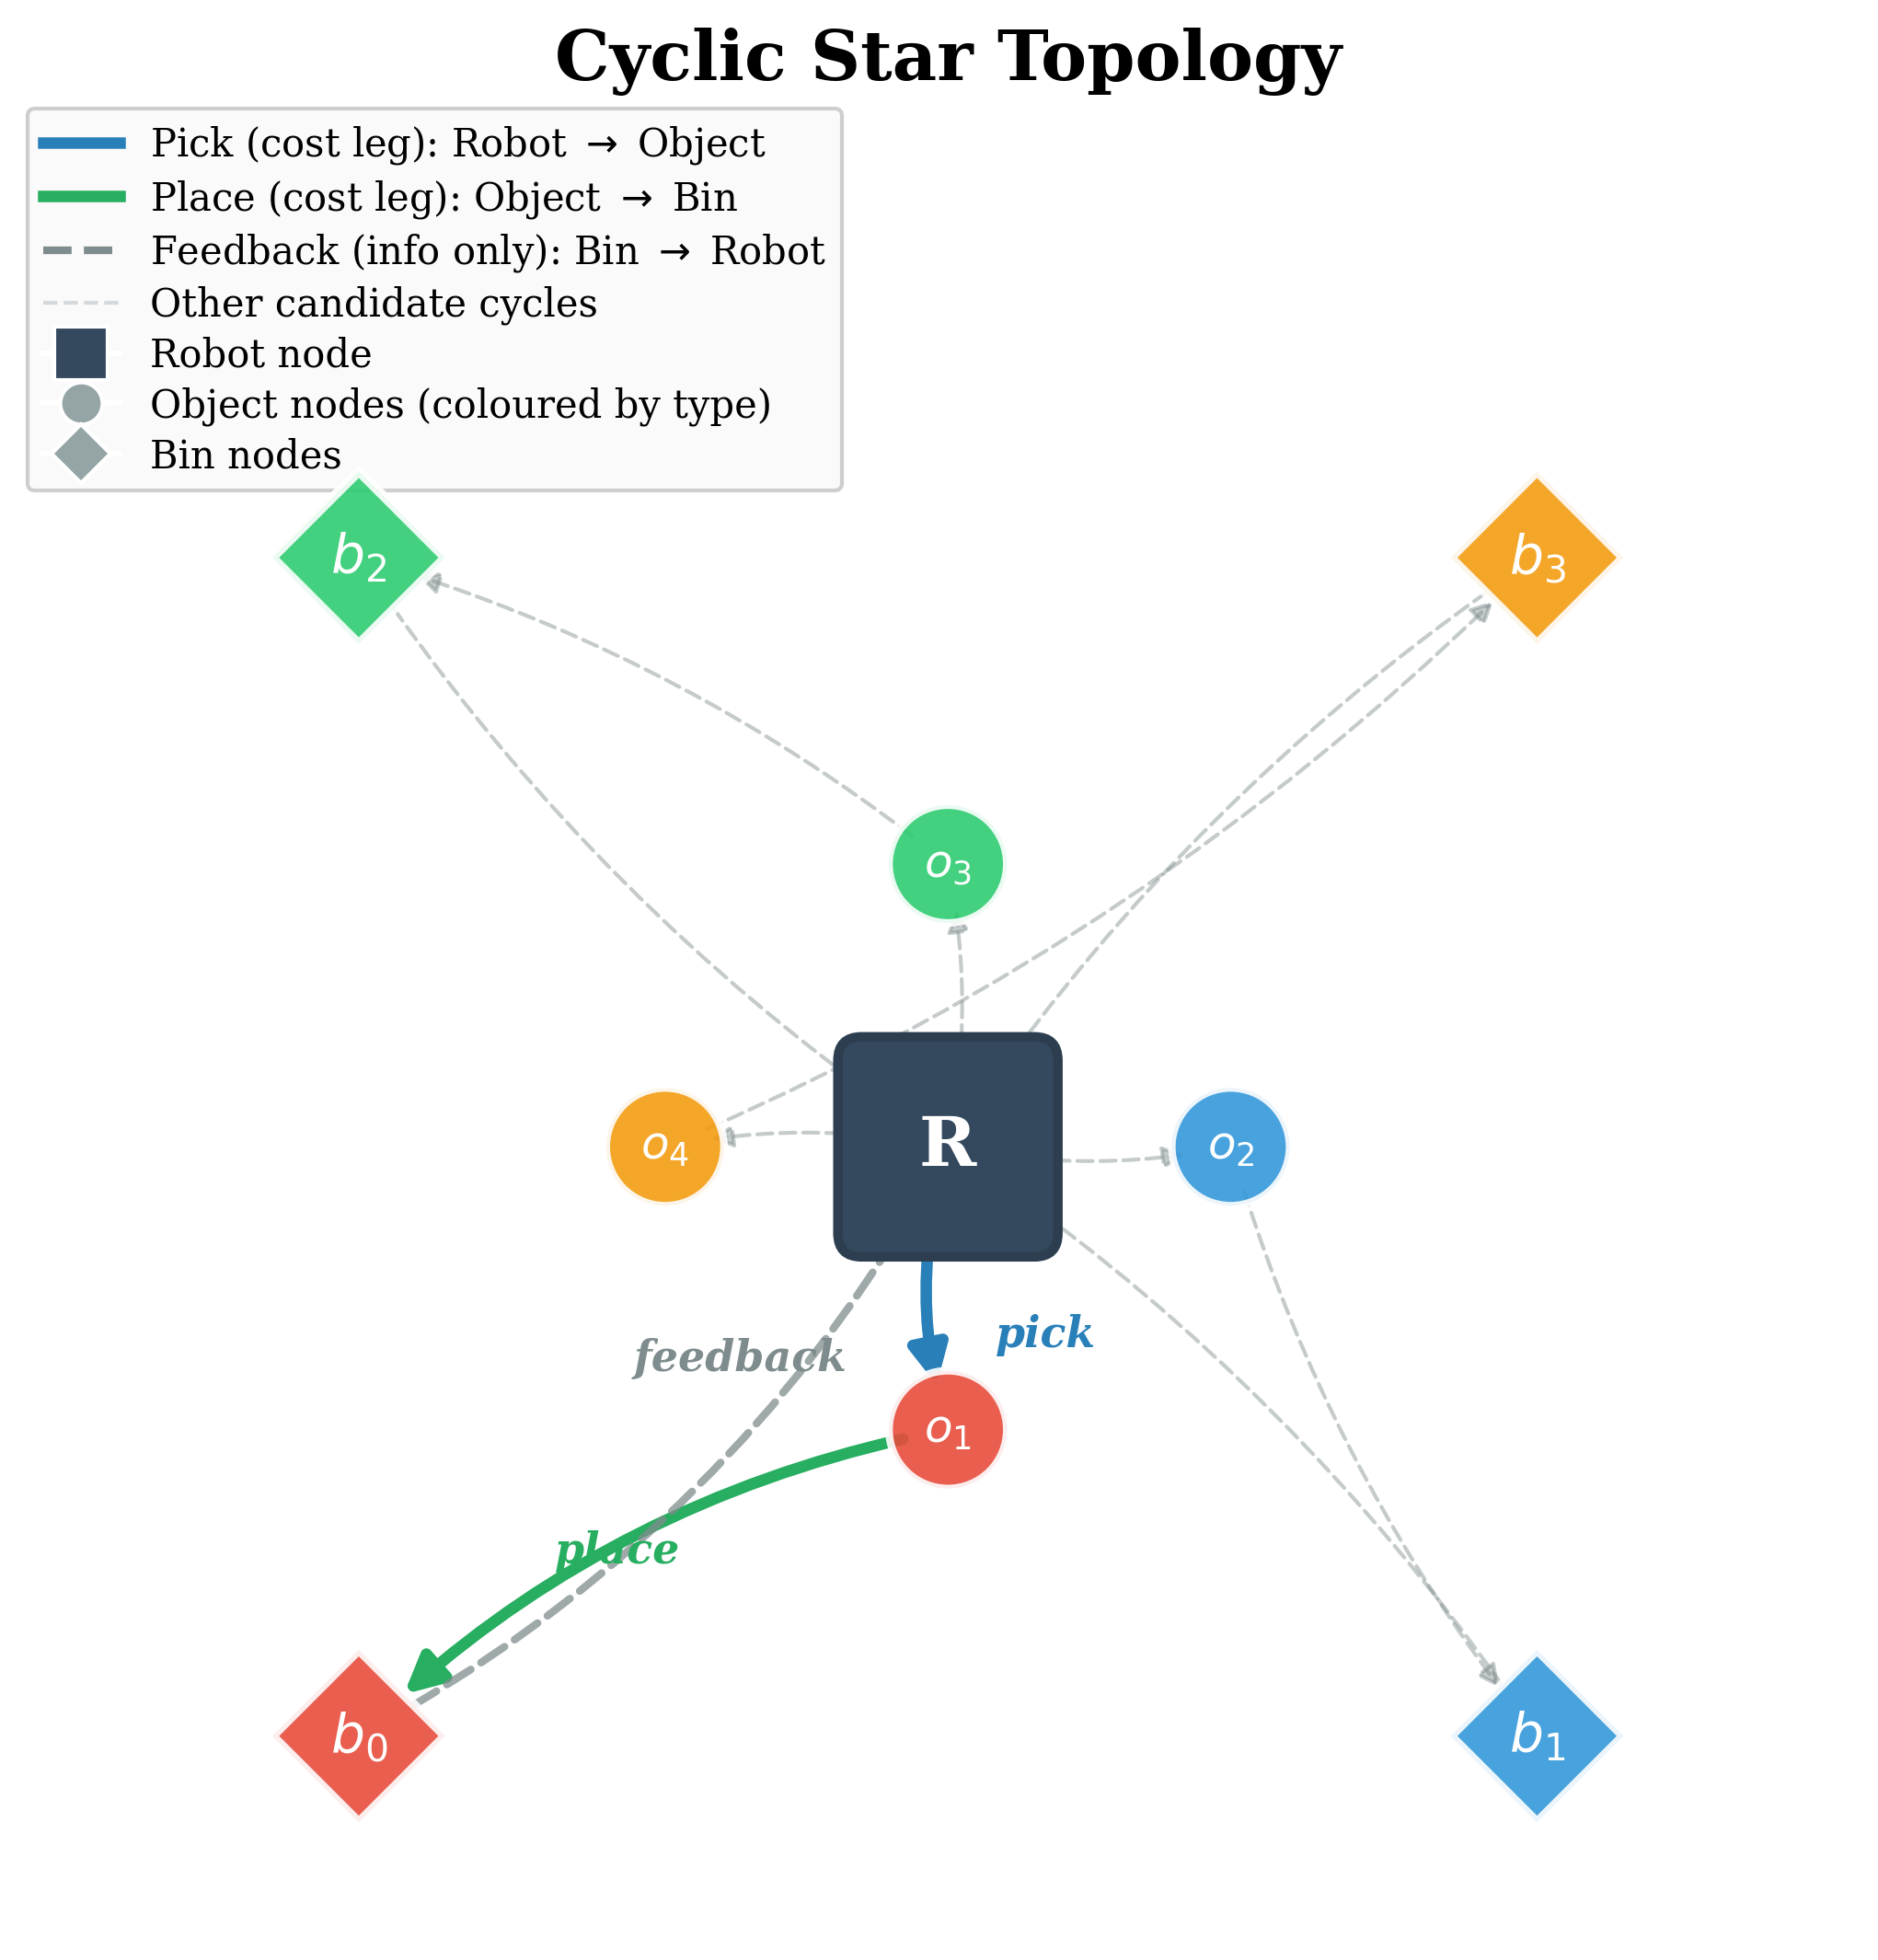
\includegraphics[width=0.9\linewidth]{figures/paper/fig1_graph_topology.png}
\caption{Cyclic star topology. Each candidate pick-and-place action corresponds to two cost-bearing directed edges (robot$\to$object pick leg in blue; object$\to$bin place leg in green) closed by a dashed bin$\to$robot feedback edge (grey) that exists only for message passing; after placement, the robot's state is set to the bin location and it moves directly to the next chosen object, so no physical return motion occurs. Three node types (robot, object, bin) carry type-encoded features processed by a standard GAT. Edges are constructed dynamically: only remaining objects participate, so the graph shrinks as the episode progresses.}
\label{fig:graph_topology}
\end{figure}

Edges are constructed only for valid objects (mask $m{=}1$), so the graph connectivity changes as objects are picked. This dynamic construction naturally represents the shrinking action space without requiring explicit re-indexing.

\subsection{Network Architecture}

Our policy $\pi_\theta$ is a Graph Attention Network (GAT). We choose GAT over GCN because the cost of picking object $i$ depends on the robot's current position, which changes at every step; GAT's learned attention coefficients $\alpha_{ij}$ adapt to this changing context, whereas GCN applies fixed aggregation weights.

The architecture consists of two \texttt{GATConv} layers (4 attention heads, \texttt{concat=False}, hidden dimension $d_h{=}128$), each followed by ReLU and dropout ($p{=}0.1$). During message passing, information propagates through the cyclic star: at each layer, the robot node aggregates from valid object nodes, each object aggregates from its assigned bin, and each bin aggregates from the robot. After two layers, each object embedding encodes information from the full cycle.

A two-layer MLP head (Linear($d_h$, $d_h$) $\to$ ReLU $\to$ Dropout $\to$ Linear($d_h$, 1)) maps each object embedding to a scalar logit. Only object node embeddings (indices $1$ through $N$) are scored:
\begin{equation}
\ell_i = \text{MLP}(h^{(L)}_{1+i}), \quad i \in \{0,\dots,N{-}1\}.
\end{equation}

The total parameter count is ${\sim}$90K, making the policy lightweight enough for embedded deployment.

\subsection{Autoregressive Inference and Masking}

The sequence is generated autoregressively. At step $t$, logits for previously picked objects are set to a large negative constant ($-10^4$) before softmax to ensure probability mass concentrates on valid actions. The action $a_t = \arg\max_i \ell_i$ is selected greedily at inference time.

\subsection{Imitation Learning with Teacher Forcing}

We treat sequencing as a classification task supervised by an expert oracle. At each step $t$, the cross-entropy loss between predicted logits and the expert's action is:
\begin{equation}
\mathcal{L}_t(\theta) = \text{CE}\big(\ell(\mathcal{G}_t;\theta),\, a_t^\star\big),
\end{equation}
with stage loss averaged over the prefix: $\mathcal{L}(\theta) = \frac{1}{P}\sum_{t=1}^{P}\mathcal{L}_t(\theta)$.

Teacher forcing updates the graph using the expert action $a_t^\star$ rather than the model's own prediction, preventing error propagation during training. This is subject to covariate shift at inference \cite{ross2011dagger}; our curriculum learning mitigates this by converging on short-horizon decisions before full-sequence rollouts.

\subsubsection{Multi-Fidelity Expert Supervision}
When available, we train on ILP-optimal prefixes. When a scenario lacks an ILP prefix at a given stage, we fall back to a greedy expert sequence. The motivation for this multi-fidelity strategy is not quality improvement (as Section~\ref{sec:ablations} (A4) shows, ILP-only supervision achieves a comparable per-scenario gap) but \emph{scale coverage}: it allows the curriculum to run at problem sizes where ILP prefixes are unavailable for most scenarios, and avoids stalling when ILP coverage at a given curriculum stage is sparse. The resulting trade-off is predictable training wall-clock time independent of the solver's per-instance completion behaviour.

\subsection{Curriculum Learning Strategy}

We implement a curriculum over prefix lengths $P \in \{5, 10, 20\}$, training sequentially from short to long horizons. Stages with $P > N$ are skipped. Earlier stages train for 3 epochs each; the final stage receives 6 epochs. This schedule allows the model to master local structure before generalising to long-horizon dependencies.

\subsection{Algorithm Summary}

Algorithm~\ref{alg:training} summarises training; Algorithm~\ref{alg:inference} summarises inference.

\begin{algorithm}[htbp]
\caption{Curriculum-Based Imitation Learning}
\label{alg:training}
\begin{algorithmic}[1]
\REQUIRE Dataset $\mathcal{D}$, prefix stages $\mathcal{P}{=}\{5,10,20\}$, ILP prefixes, greedy fallback
\ENSURE Trained policy $\pi_\theta$
\STATE Initialise GAT policy (2 layers, $d_h{=}128$, 4 heads)
\STATE Initialise AdamW ($\alpha{=}10^{-3}$, $\lambda{=}10^{-2}$, $\beta{=}(0.9, 0.95)$)
\STATE Initialise cosine LR scheduler
\FOR{each stage $P \in \mathcal{P}$ (skip if $P > N$)}
    \STATE $E_P \leftarrow 3$ if $P \neq \max(\mathcal{P})$ else $6$
    \STATE Collect stage set: ILP prefix at $P$, else greedy fallback
    \FOR{epoch $= 1$ to $E_P$}
        \FOR{each scenario $s$ (random order)}
            \STATE Retrieve expert prefix $(a_1^\star, \dots, a_P^\star)$
            \FOR{$t = 1$ to $P$}
                \STATE Build $\mathcal{G}_t$; compute $\ell \leftarrow \pi_\theta(\mathcal{G}_t)$
                \STATE $\mathcal{L}_t \leftarrow \text{CE}(\ell, a_t^\star)$; update state
            \ENDFOR
            \STATE Backpropagate $\frac{1}{P}\sum_t \mathcal{L}_t$; clip $\|\nabla\|{\le}1.0$; step
        \ENDFOR
        \STATE Evaluate; save if best gap vs.\ greedy
    \ENDFOR
\ENDFOR
\end{algorithmic}
\end{algorithm}

\begin{algorithm}[htbp]
\caption{Greedy Inference Rollout}
\label{alg:inference}
\begin{algorithmic}[1]
\REQUIRE Trained $\pi_\theta$, scenario with $N$ objects
\ENSURE Sequence $(a_1, \dots, a_N)$, cost $C$
\STATE $r_0 \leftarrow \text{start}$; mask $\leftarrow \mathbf{1}_N$; $C \leftarrow 0$
\FOR{$t = 1$ to $N$}
    \STATE Build $\mathcal{G}_t$; $\ell \leftarrow \pi_\theta(\mathcal{G}_t)$
    \STATE $a_t \leftarrow \arg\max_i \ell_i$
    \STATE $C \leftarrow C + \|r_t - o_{a_t}\| + \|o_{a_t} - b_{\tau(a_t)}\|$
    \STATE mask[$a_t$] $\leftarrow 0$; $r_{t+1} \leftarrow b_{\tau(a_t)}$
\ENDFOR
\end{algorithmic}
\end{algorithm}

\subsection{Training Details}

Optimisation uses AdamW \cite{loshchilov2019adamw} with $\alpha{=}10^{-3}$, weight decay $10^{-2}$, $\beta{=}(0.9, 0.95)$, gradient clipping at norm 1.0, cosine annealing over total updates, and a 90/10 train/validation split with fixed seed. Gradient accumulation over 8 scenarios stabilises updates across variable-size graphs. Fig.~\ref{fig:training_loss} and Fig.~\ref{fig:training_cost} show the training loss and validation cost progression under the curriculum.

\begin{figure}
    \centering
    
\includegraphics[width=0.9\linewidth]{figures/40obj/training/loss.png}
    \caption{Cross-entropy loss over 12 epochs, coloured by curriculum stage.}
    \label{fig:training_loss}
\end{figure}
\begin{figure}
    \centering
    
\includegraphics[width=0.9\linewidth]{figures/40obj/training/val_cost.png}
    \caption{Validation cost comparison ($N{=}40$). The GNN cost drops below the Greedy baseline by epoch 2 and continues improving.}
    \label{fig:training_cost}
\end{figure}
\begin{figure}
    \centering
    
\includegraphics[width=0.9\linewidth]{figures/40obj/training/win_rate.png}
    \caption{Validation win-rate vs.\ Greedy during training ($N{=}40$). The model surpasses 90\% win-rate after the first curriculum stage transition and stabilises at 96--99\%.}
    \label{fig:training_win_rate}
\end{figure}


\subsection{Evaluation Metrics}

We report: (i) \textbf{gap vs.\ greedy} $= (\text{greedy} - \text{model}) / \text{greedy} \times 100\%$ (positive = GNN better); (ii) \textbf{gap vs.\ ILP} (analogous, when available); (iii) \textbf{win-rate} (fraction of scenarios where GNN cost $<$ greedy cost). Inference complexity for a full $N$-object rollout is $O(N^2)$ due to the shrinking sparse graph (per-step work sums to $N(N{+}1)/2$).

%========================================================================
\section{Dataset and Experimental Setup}\label{sec:data}
%========================================================================

\subsection{Scope and Generation}

We generated 5{,}000 scenarios per object count $N \in \{3, 5, 10, 20, 40, 100, 200\}$ via procedural generation. The workspace is a $100 \times 100$ plane with four bins at corners $\{(10,10), (90,10), (10,90), (90,90)\}$. Object positions, types (0--3), and robot start poses are sampled uniformly at random. All scenarios are generated using fixed random seeds (seed equal to scenario index) to ensure reproducibility and consistent evaluation across methods.

\subsection{Offline Expert Annotation}

ILP-optimal prefixes are pre-computed offline at lengths the solver handles within a timeout budget. Smaller instances ($N{\le}10$) admit full-length ILP solutions; larger instances yield shorter prefixes. Greedy nearest-cycle (NC) baselines are computed for every scenario. Both are embedded in the dataset schema alongside spatial data, enabling training without online solver calls.

\subsection{Data Schema}

Each scenario is serialised in JSON with fields: \texttt{objects} ($(x,y)$ coordinates), \texttt{types} (bin assignments), \texttt{bins}, \texttt{start}, \texttt{greedy\_sequence}, \texttt{greedy\_cost}, \texttt{ilp\_prefixes} (keyed by prefix length), and \texttt{ilp\_costs}. A sample is shown in Fig.~\ref{fig:json_sample}.

\begin{figure}[htbp]
\centering
\begin{scriptsize}
\begin{verbatim}
{
  "objects": [[53.9, 67.2], [58.2, 53.5], ...],
  "types": [2, 3, 0, 1, 3, 1, 3, 3, 2, 3],
  "bins": [[10,10], [90,10], [10,90], [90,90]],
  "start": [61.19, 21.47],
  "greedy_sequence": [5, 4, 9, 6, 0, 8, 2, 7, 1, 3],
  "greedy_cost": 835.21,
  "ilp_prefixes": {"5": [1,3,4,0,2], "10": [...]},
  "ilp_costs": {"5": 489.09, "10": 827.20}
}
\end{verbatim}
\end{scriptsize}
\caption{Truncated dataset schema for a 10-object scenario.}
\label{fig:json_sample}
\end{figure}

%========================================================================
\section{Results}\label{sec:results}
%========================================================================

We evaluate the GNN policy on held-out validation sets. For each $N$, 5{,}000 scenarios were generated; the model trained on 4{,}500 and evaluated on 100 held-out validation scenarios. The dataset is split into 90\% training and 10\% validation scenarios using a fixed random seed with no overlap, ensuring that all reported results are evaluated on unseen instances. All evaluations use the same 100-scenario validation set per problem size for consistency across tables and figures.

\subsection{Cost Comparison vs.\ Baselines}

Table~\ref{tab:results_40obj} shows the GNN produces consistently lower mean travel cost than Greedy on $N{=}40$, with lower variance. The 98.0\% win-rate confirms this is not driven by outliers.

\begin{table}[htbp]
\caption{Evaluation results ($N{=}40$, 100 validation scenarios). Positive $\Delta$ indicates GNN is better (lower cost).}
\label{tab:results_40obj}
\centering
\begin{tabular}{@{}lccc@{}}
\toprule
\textbf{Method} & \textbf{Mean Cost} & \textbf{Std} & \textbf{$\Delta$ vs Greedy} \\
\midrule
GNN (ours) & 3773.1 & 176.7 & +3.23\% \\
Greedy & 3899.5 & 177.4 & \multicolumn{1}{c}{---} \\
\bottomrule
\end{tabular}

\vspace{2mm}
\begin{tabular}{@{}lc@{}}
\toprule
\textbf{Win-rate} & \textbf{Value} \\
\midrule
GNN beats Greedy & 98/100 (98.0\%) \\
\bottomrule
\end{tabular}
\end{table}

\begin{figure}[htbp]
\centering

\includegraphics[width=0.9\linewidth]{figures/40obj/evaluation/scatter_gnn_vs_greedy.png}
\caption{Per-scenario cost comparison ($N{=}40$, 100 scenarios). Points below the diagonal indicate GNN improvement. The GNN produces lower cost in 98 of 100 scenarios.}
\label{fig:scatter}
\end{figure}

\begin{figure}[htbp]
\centering

\includegraphics[width=0.9\linewidth]{figures/40obj/evaluation/cdf_improvement.png}
\caption{Cumulative distribution of per-scenario improvement over Greedy ($N{=}40$, 100 scenarios). 98\% of scenarios fall above zero, and 50\% of scenarios show at least 3.21\% improvement.}
\label{fig:cdf}
\end{figure}

\subsection{Optimality Gap to ILP}

Table~\ref{tab:ilp_gap} reports per-sample ILP gaps on $N{=}10$, where exact ILP optima are tractable to compute and the dataset includes the optimum cost for every scenario. We re-target this table from $N{=}40$ to $N{=}10$ because exact CBC ILP at $N{=}40$ exceeds practical wall-clock budgets ($>$60\,s per instance with no solution returned). The 10 scenarios are evenly spaced by greedy cost across the full validation set to span the difficulty range. The GNN matches ILP exactly on the easiest instance and achieves a mean gap of 1.51\% with a worst-case of 5.51\%. Across the 100-scenario validation set at $N{=}10$, the GNN achieves a mean gap to ILP of 1.81\% (Table~\ref{tab:cross_size}) and a mean improvement of 5.81\% over greedy.

\begin{table}[htbp]
\caption{Per-sample optimality gap ($N{=}10$, 10 validation scenarios evenly spaced by greedy cost across the difficulty range). ILP costs are stored exact optima from the dataset; GNN costs are produced by the trained \texttt{gnn\_10obj\_best.pt} checkpoint (the same model whose aggregate numbers populate Table~\ref{tab:cross_size}).}
\label{tab:ilp_gap}
\centering
\begin{tabular}{@{}cccc@{}}
\toprule
\textbf{S} & \textbf{GNN Cost} & \textbf{ILP Cost} & \textbf{Gap} \\
\midrule
1  & 667.18 & 667.18 & 0.00\% \\
2  & 853.31 & 840.45 & 1.53\% \\
3  & 939.00 & 927.35 & 1.26\% \\
4  & 832.23 & 818.84 & 1.63\% \\
5  & 959.52 & 953.64 & 0.62\% \\
6  & 1004.16 & 1003.51 & 0.06\% \\
7  & 1081.61 & 1025.15 & 5.51\% \\
8  & 1089.79 & 1066.80 & 2.16\% \\
9  & 1099.73 & 1076.90 & 2.12\% \\
10 & 1212.65 & 1209.96 & 0.22\% \\
\bottomrule
\end{tabular}
\vspace{1mm}
\footnotesize ILP costs are stored full-$N$ optima from the dataset (CBC offline annotation). GNN inference timing is reported separately in Fig.~\ref{fig:timing_scaling} and Table~\ref{tab:cross_size}.
\end{table}

\begin{figure}[htbp]
\centering

\includegraphics[width=\linewidth]{figures/route_examples/10_objects/scenario_2264/gnn.png}
\caption{GNN route on a representative 10-object validation scenario (median improvement case, +4.68\% vs.\ greedy NC). Pick legs are drawn in blue; place legs are coloured by target bin. Compare to the ILP-optimal route in Fig.~\ref{fig:route_ilp}.}
\label{fig:route_gnn}
\end{figure}

\begin{figure}[htbp]
\centering

\includegraphics[width=\linewidth]{figures/route_examples/10_objects/scenario_2264/ilp.png}
\caption{ILP-optimal route on the same 10-object validation scenario as Fig.~\ref{fig:route_gnn}. The GNN's sequence (cost 953.5) closely tracks the ILP-optimal sequence (cost 916.0), confirming successful distillation at scales where the teacher is available.}
\label{fig:route_ilp}
\end{figure}

\subsection{Inference Time Scaling}\label{sec:timing}

A key operational advantage is \emph{predictable} inference time. ILP solve time grows exponentially with $N$ and frequently exceeds real-time budgets: at $N{=}40$, all instances exceed a 60\,s timeout. GNN inference scales polynomially with graph size, yielding consistent median runtimes: 26\,ms at $N{=}10$, 125\,ms at $N{=}40$, and 960\,ms at $N{=}200$ (NVIDIA RTX~2050 GPU with CUDA synchronisation, 100 validation scenarios, 10 warmup passes). For comparison, Greedy runs in 0.02--8.3\,ms across the same range. Fig.~\ref{fig:timing_scaling} visualises this scaling behaviour.

\begin{figure}[htbp]
\centering
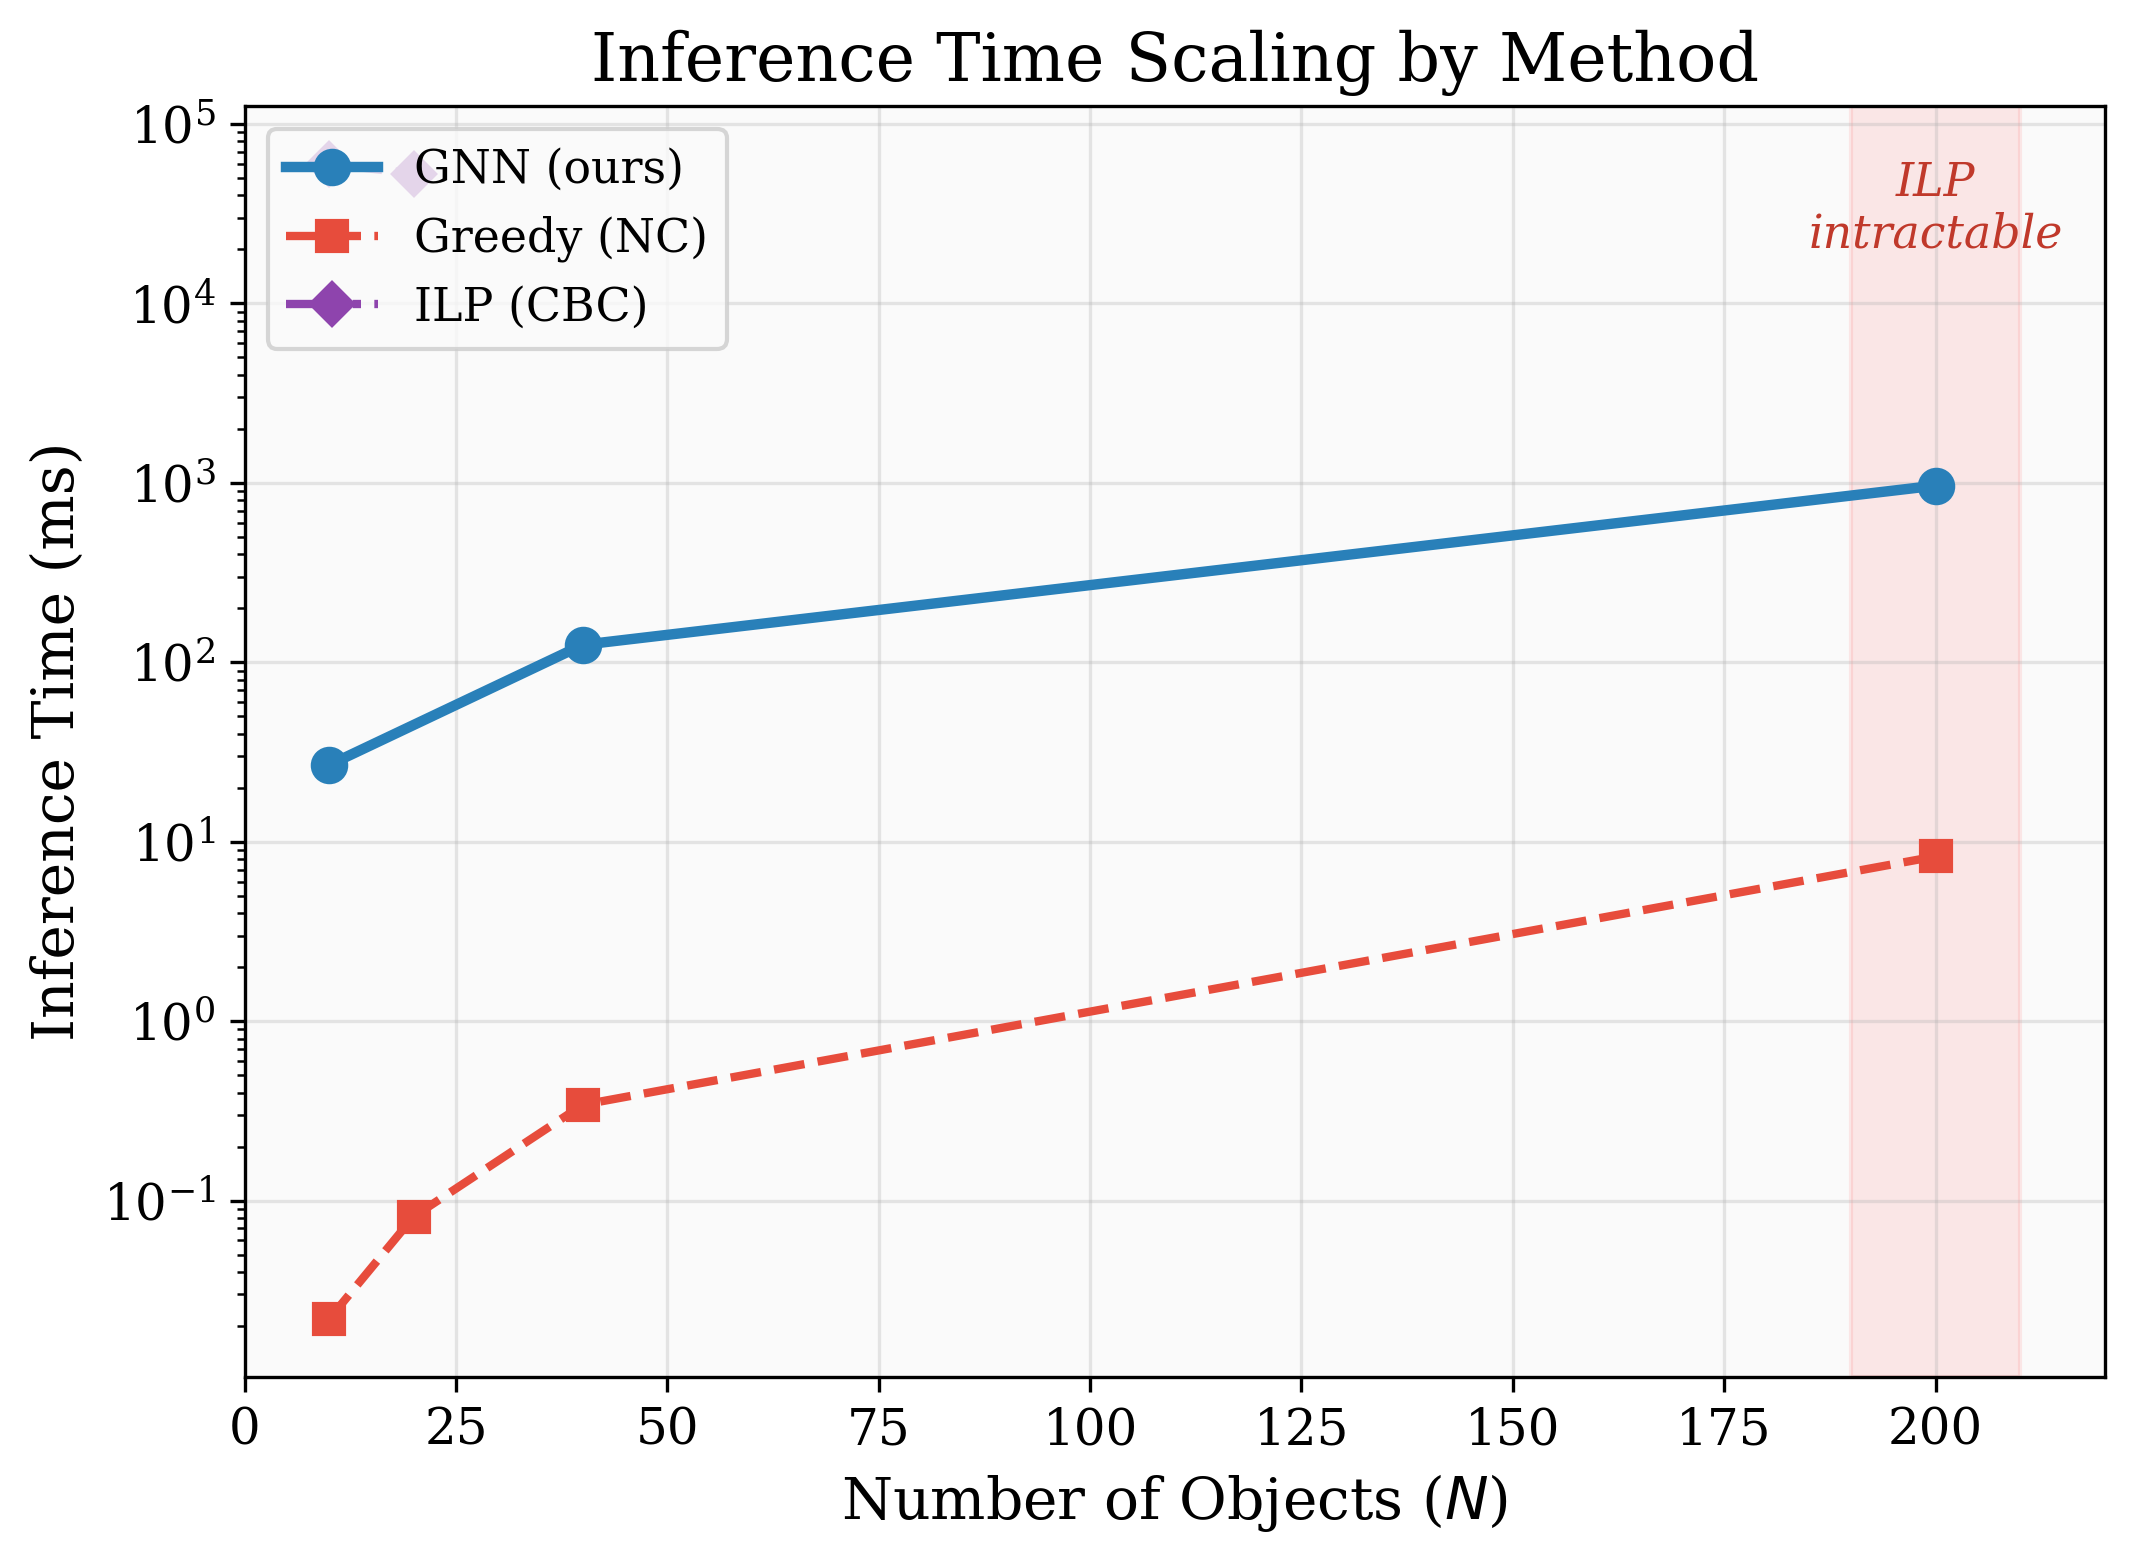
\includegraphics[width=0.9\linewidth]{figures/paper/fig_timing_scaling.png}
\caption{Inference time scaling (log-scale). GNN inference grows polynomially with $N$, while ILP is intractable beyond $N{\approx}40$. Greedy is fastest but sacrifices solution quality. GNN runtime variability is low: std = 2.5\,ms (p95 = 31\,ms) at $N{=}10$; std = 6.0\,ms (p95 = 135\,ms) at $N{=}40$; std = 41\,ms (p95 = 1050\,ms) at $N{=}200$. At $N{=}10$, only 13 of 50 ILP instances solved within a 60\,s CPU timeout.}
\label{fig:timing_scaling}
\end{figure}

For $N{=}100$ and $N{=}200$, ILP is entirely intractable; the GNN provides the only near-optimal baseline, demonstrating the scalability payoff of solver distillation. Table~\ref{tab:results_200obj} confirms this: at $N{=}200$, the GNN improves on Greedy in 100\% of scenarios (100/100) with a mean improvement of 1.67\%.

\begin{table}[htbp]
\caption{Evaluation results ($N{=}200$, 100 validation scenarios).}
\label{tab:results_200obj}
\centering
\begin{tabular}{@{}lccc@{}}
\toprule
\textbf{Method} & \textbf{Mean Cost} & \textbf{Std} & \textbf{$\Delta$ vs Greedy} \\
\midrule
GNN (ours) & 18544.2 & 308.3 & +1.67\% \\
Greedy & 18860.2 & 364.7 & \multicolumn{1}{c}{---} \\
\bottomrule
\end{tabular}

\vspace{2mm}
\begin{tabular}{@{}lc@{}}
\toprule
\textbf{Win-rate} & \textbf{Value} \\
\midrule
GNN beats Greedy & 100/100 (100\%) \\
\bottomrule
\end{tabular}
\end{table}

\subsection{Cost Comparison Across Problem Sizes}

Table~\ref{tab:cross_size} summarises performance across all evaluated sizes. The GNN outperforms Greedy with win-rates $\geq$90.8\% at every scale. At $N{=}20$ (full ILP available), the mean gap to ILP is only 1.40\%.

\begin{table}[htbp]
\caption{GNN vs.\ Greedy across problem sizes (100 validation scenarios each).}
\label{tab:cross_size}
\centering
\begin{tabular}{@{}lcccc@{}}
\toprule
& $N{=}10$ & $N{=}20$ & $N{=}40$ & $N{=}200$ \\ 
\midrule
GNN mean cost        & 971   & 1905  & 3773  & 18544 \\
Greedy mean cost     & 1032  & 2003  & 3900  & 18860 \\
Gap vs.\ Greedy (\%)     & 5.81  & 4.88  & 3.23  & 1.67 \\
Gap std (\%)         & 5.64  & 3.13  & 1.85  & 0.82 \\
Win-rate (\%)        & 90.8    & 100   & 98    & 100 \\
Gap vs.\ ILP (\%)   & 1.81  & 1.40  & ---$^{\ddag}$ & --- \\
\bottomrule
\end{tabular}
\vspace{1mm}

\footnotesize The $N{=}10$ and $N{=}20$ ILP gaps are computed using pre-computed optimal costs cached in the dataset. $^{\ddag}$$N{=}40$ ILP is intractable for per-sample optima (CBC exceeds 60\,s with no solution returned); see Table~\ref{tab:ilp_gap} which reports per-sample gaps at $N{=}10$. GNN inference timing is reported in Fig.~\ref{fig:timing_scaling}.
\end{table}

Fig.~\ref{fig:cost_comparison} visualises the cost comparison.

\begin{figure}[htbp]
    \centering
    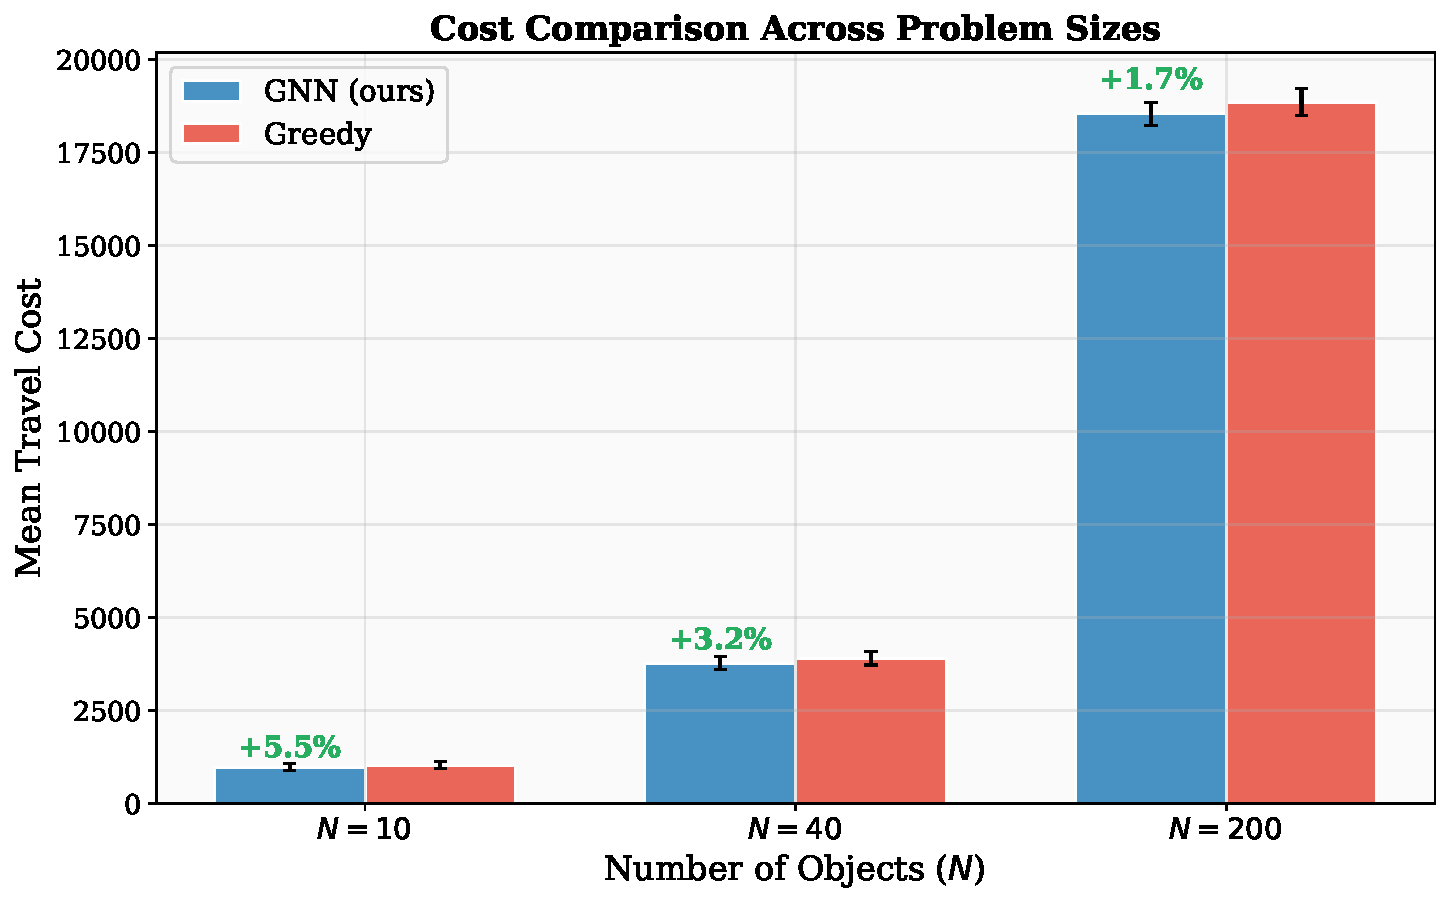
\includegraphics[width=0.9\linewidth]{figures/paper/fig2_cost_comparison.pdf}
    \caption{Travel cost comparison across problem sizes ($N \in \{10, 40, 200\}$) for GNN and Greedy. Lower is better. Percentage labels indicate GNN improvement over Greedy.}
    \label{fig:cost_comparison}
\end{figure}

\begin{figure}[htbp]
    \centering
    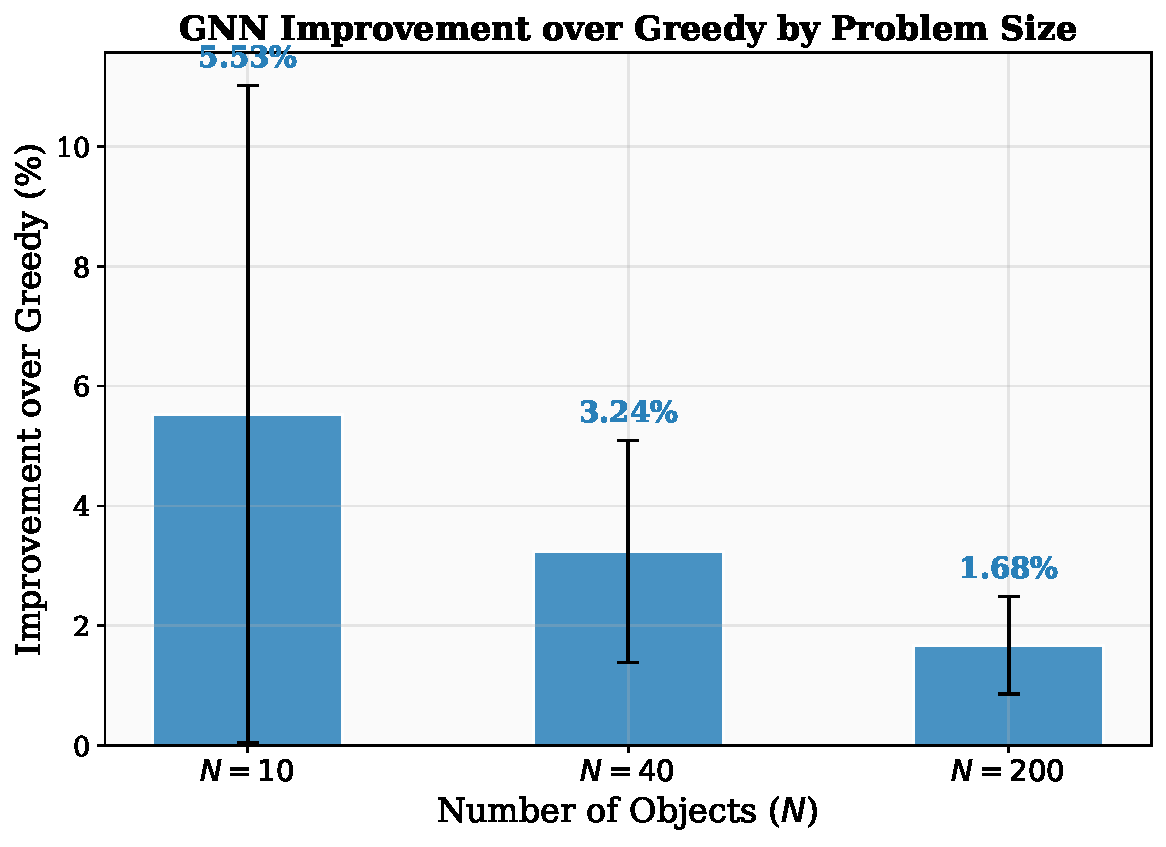
\includegraphics[width=0.9\linewidth]{figures/paper/fig2_gap_by_size.pdf}
    \caption{Mean GNN improvement over Greedy (\%) by problem size. Error bars show per-scenario standard deviation. The advantage is largest at $N{=}10$ (5.81\%) and decreases with scale, but remains positive at $N{=}200$ (1.67\%).}
    \label{fig:gap_by_size}
\end{figure}

\begin{figure}[htbp]
\centering

\includegraphics[width=0.9\linewidth]{figures/40obj/evaluation/difficulty_breakdown.png}
\caption{GNN vs.\ Greedy cost by scenario difficulty ($N{=}40$, 100 scenarios). Scenarios are binned by Greedy cost (proxy for difficulty). The GNN advantage is consistent across easy and hard scenarios.}
\label{fig:difficulty}
\end{figure}

\subsection{Statistical Analysis}\label{sec:stats}

To establish the reliability of our results, we report paired significance testing and bootstrap confidence intervals computed over the 100-scenario validation set.

\subsubsection{Significance Testing}

We perform a paired $t$-test comparing GNN cost vs.\ greedy cost on each of the 100 validation scenarios (pairing by scenario). The null hypothesis that the two methods produce equal mean costs is rejected with $p < 10^{-31}$, confirming the improvement is not attributable to chance. A 95\% bootstrap confidence interval for the mean improvement is [2.88\%, 3.59\%].

\subsubsection{Distribution of Improvements}

Fig.~\ref{fig:boxplot} shows the distribution of per-scenario cost improvements (GNN cost $-$ greedy cost) across the 100-scenario validation set, visualised as box plots for each $N$.

\begin{figure}[htbp]
\centering
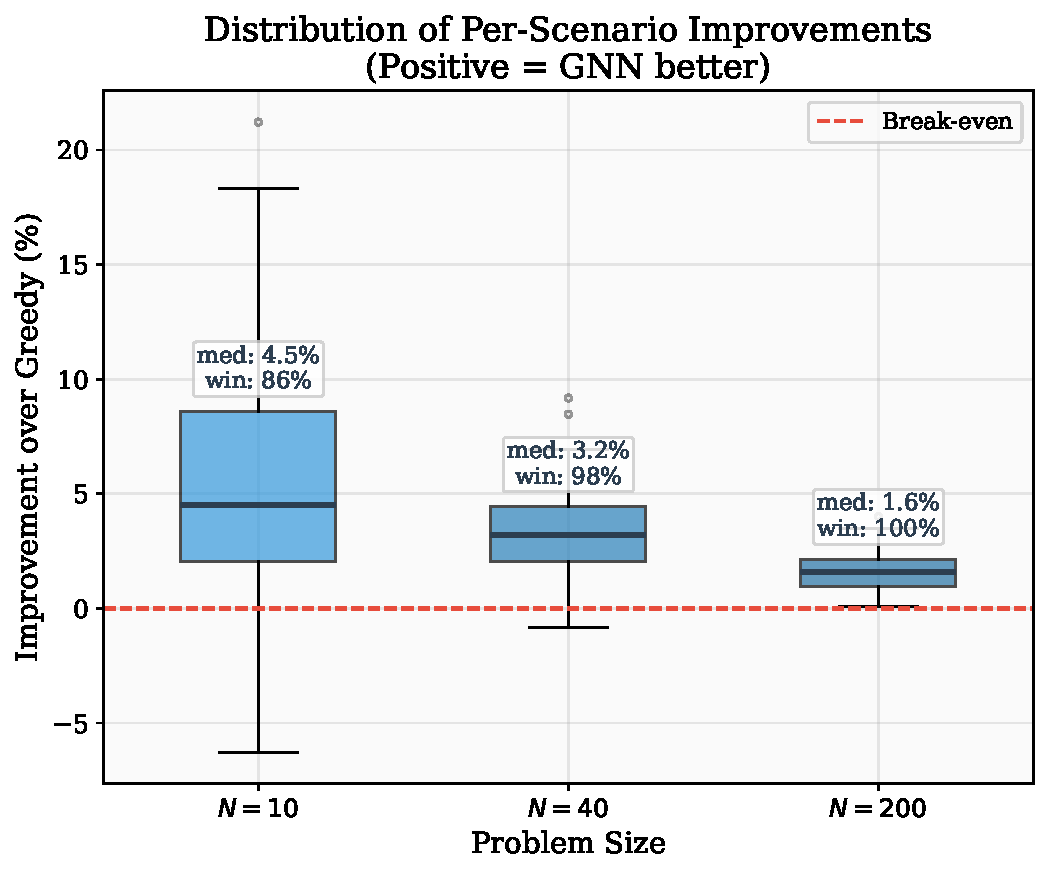
\includegraphics[width=0.9\linewidth]{figures/paper/fig3_boxplot_gap_pct.pdf}
\caption{Distribution of per-scenario improvements (Greedy $-$ GNN / Greedy, \%). Boxes show median and interquartile range; whiskers extend to 1.5$\times$IQR. Positive values indicate GNN is better.}
\label{fig:boxplot}
\end{figure}

\begin{figure}[htbp]
\centering

\includegraphics[width=0.9\linewidth]{figures/40obj/steps/per_step_advantage.png}
\caption{Per-step cost advantage ($N{=}40$, averaged over 50 scenarios). The GNN sacrifices cost in early steps (mean $-$11.3) but dominates late-sequence steps (mean $+$19.0), confirming multi-step lookahead rather than single-step mimicry.}
\label{fig:step_advantage}
\end{figure}

\begin{figure}[htbp]
\centering

\includegraphics[width=0.9\linewidth]{figures/40obj/routes/best_win_gnn.png}

\includegraphics[width=0.9\linewidth]{figures/40obj/routes/best_win_greedy.png}
\caption{Route visualisation for the scenario with largest GNN advantage ($N{=}40$). Top: GNN route. Bottom: Greedy route. Arrows show pick (blue) and place (coloured by bin type) legs. The GNN produces fewer cross-workspace traversals.}
\label{fig:route_example}
\end{figure}

\begin{figure}[htbp]
\centering

\includegraphics[width=0.9\linewidth]{figures/40obj/evaluation/histogram_improvement.png}
\caption{Histogram of per-scenario improvement over Greedy ($N{=}40$, 100 scenarios). The distribution is approximately normal with mean 3.23\% and median 3.21\%. Only 2 of 100 scenarios show greedy outperforming the GNN.}
\label{fig:histogram}
\end{figure}

\subsection{Ablation Study}\label{sec:ablations}

We isolate the contribution of each design choice via controlled ablations on $N{=}40$ (900 training / 100 validation scenarios). Each ablation modifies one component while holding others fixed. Table~\ref{tab:ablations} reports the best mean gap vs.\ greedy achieved by each variant.

\begin{table}[htbp]
\caption{Ablation study ($N{=}40$, 100 val scenarios). Gap vs.\ greedy (\%): positive = better than greedy. Win-rate: fraction of scenarios where model beats greedy. Ablations use the same 100-scenario split as the main evaluation (Table~\ref{tab:results_40obj}) but train on a reduced 900-scenario training set; absolute gaps differ slightly but the ranking of variants is consistent.}
\label{tab:ablations}
\centering
\begin{tabular}{@{}llcc@{}}
\toprule
\textbf{Ablation} & \textbf{Variant} & \textbf{Gap (\%)} & \textbf{Win (\%)} \\
\midrule
\multirow{3}{*}{A1: Graph}
    & Cyclic star (ours) & +2.59 & 93.0 \\
    & Fully connected & $-$24.8 & 0.0 \\
    & $k$-NN ($k{=}5$) & +0.79 & 62.0 \\
\cmidrule(l){2-4}
\multirow{3}{*}{A2: Encoder}
    & GAT (ours) & +2.59 & 93.0 \\
    & GCN & $-$0.51 & 38.0 \\
    & MLP (no graph) & $-$24.2 & 0.0 \\
\cmidrule(l){2-4}
\multirow{2}{*}{A3: Curriculum}
    & Curriculum (ours) & +2.59 & 93.0 \\
    & No curriculum & +0.22 & 52.0 \\
\cmidrule(l){2-4}
\multirow{3}{*}{A4: Supervision}
    & ILP + Greedy (ours) & +2.59 & 93.0 \\
    & ILP-only & +3.00 & 92.0 \\
    & Greedy-only & $-$1.31 & 29.0 \\
\bottomrule
\end{tabular}
\end{table}

\textbf{A1 (Graph structure):} The fully connected graph fails catastrophically ($-$24.8\% gap, 0\% win-rate), producing costs indistinguishable from an untrained policy. A follow-up extended-budget re-run (3$\times$ the original epochs per stage) produced essentially identical results ($-$24.98\% for FC, $-$24.26\% for MLP; see A2), confirming that the failure is \emph{structural} rather than a training-budget artefact. The likely mechanism is that $O(N^2)$ undirected edges dilute attention over the task-relevant pick-place cycles, so the correct structural signal never dominates the aggregated messages. The $k$-NN graph (+0.79\%, 62\%) does learn a weak policy but is substantially weaker than the cyclic star (+2.59\%, 93\%) at $N{=}40$, where bin placement creates long-range dependencies that spatial locality alone cannot capture.

\textbf{A2 (Encoder):} GAT outperforms GCN (+2.59\% vs.\ $-$0.51\%) because learned attention weights adapt to the robot's changing position, while GCN's fixed aggregation cannot. MLP (no graph) also fails catastrophically ($-$24.2\%), matching the FC result and confirming that both variants reach the same failure mode: absence of the cyclic pick-place inductive bias prevents the model from learning any sequencing signal within the fixed training budget. This is a shared structural pathology, not two independent architectural deficiencies, and the interpretation is that relational reasoning with the correct topology (not merely ``some graph'') is what delivers the advantage.

\textbf{A3 (Curriculum):} Curriculum learning is critical for training efficiency at $N{=}40$: the curriculum variant achieves +2.59\% gap (93\% win-rate) while the no-curriculum variant reaches only +0.22\% (52\% win-rate) given the same total training budget. By mastering short-horizon structure before long 40-step sequences, the curriculum enables faster convergence within a fixed epoch budget.

\textbf{A4 (Supervision):} Greedy-only supervision fails to beat greedy ($-$1.31\%, 29\% win-rate), confirming that ILP teacher quality is essential for learning non-myopic decisions. ILP-only supervision (+3.00\%, 92\% win) and mixed ILP+Greedy (+2.59\%, 93\% win) are statistically comparable on per-scenario gap; the mixed variant's trailing 0.41-percentage-point deficit is within the noise of a 100-scenario ablation split. The reason to prefer the mixed variant is therefore not gap quality but operational: it enables training to proceed on scenarios where ILP prefixes are absent (inevitable at $N{\ge}40$ where the solver exceeds its timeout on most instances) without stalling the curriculum schedule. ILP-only is a valid alternative when full prefix coverage is available, and either strategy strictly dominates greedy-only supervision.

\begin{figure}[htbp]
\centering
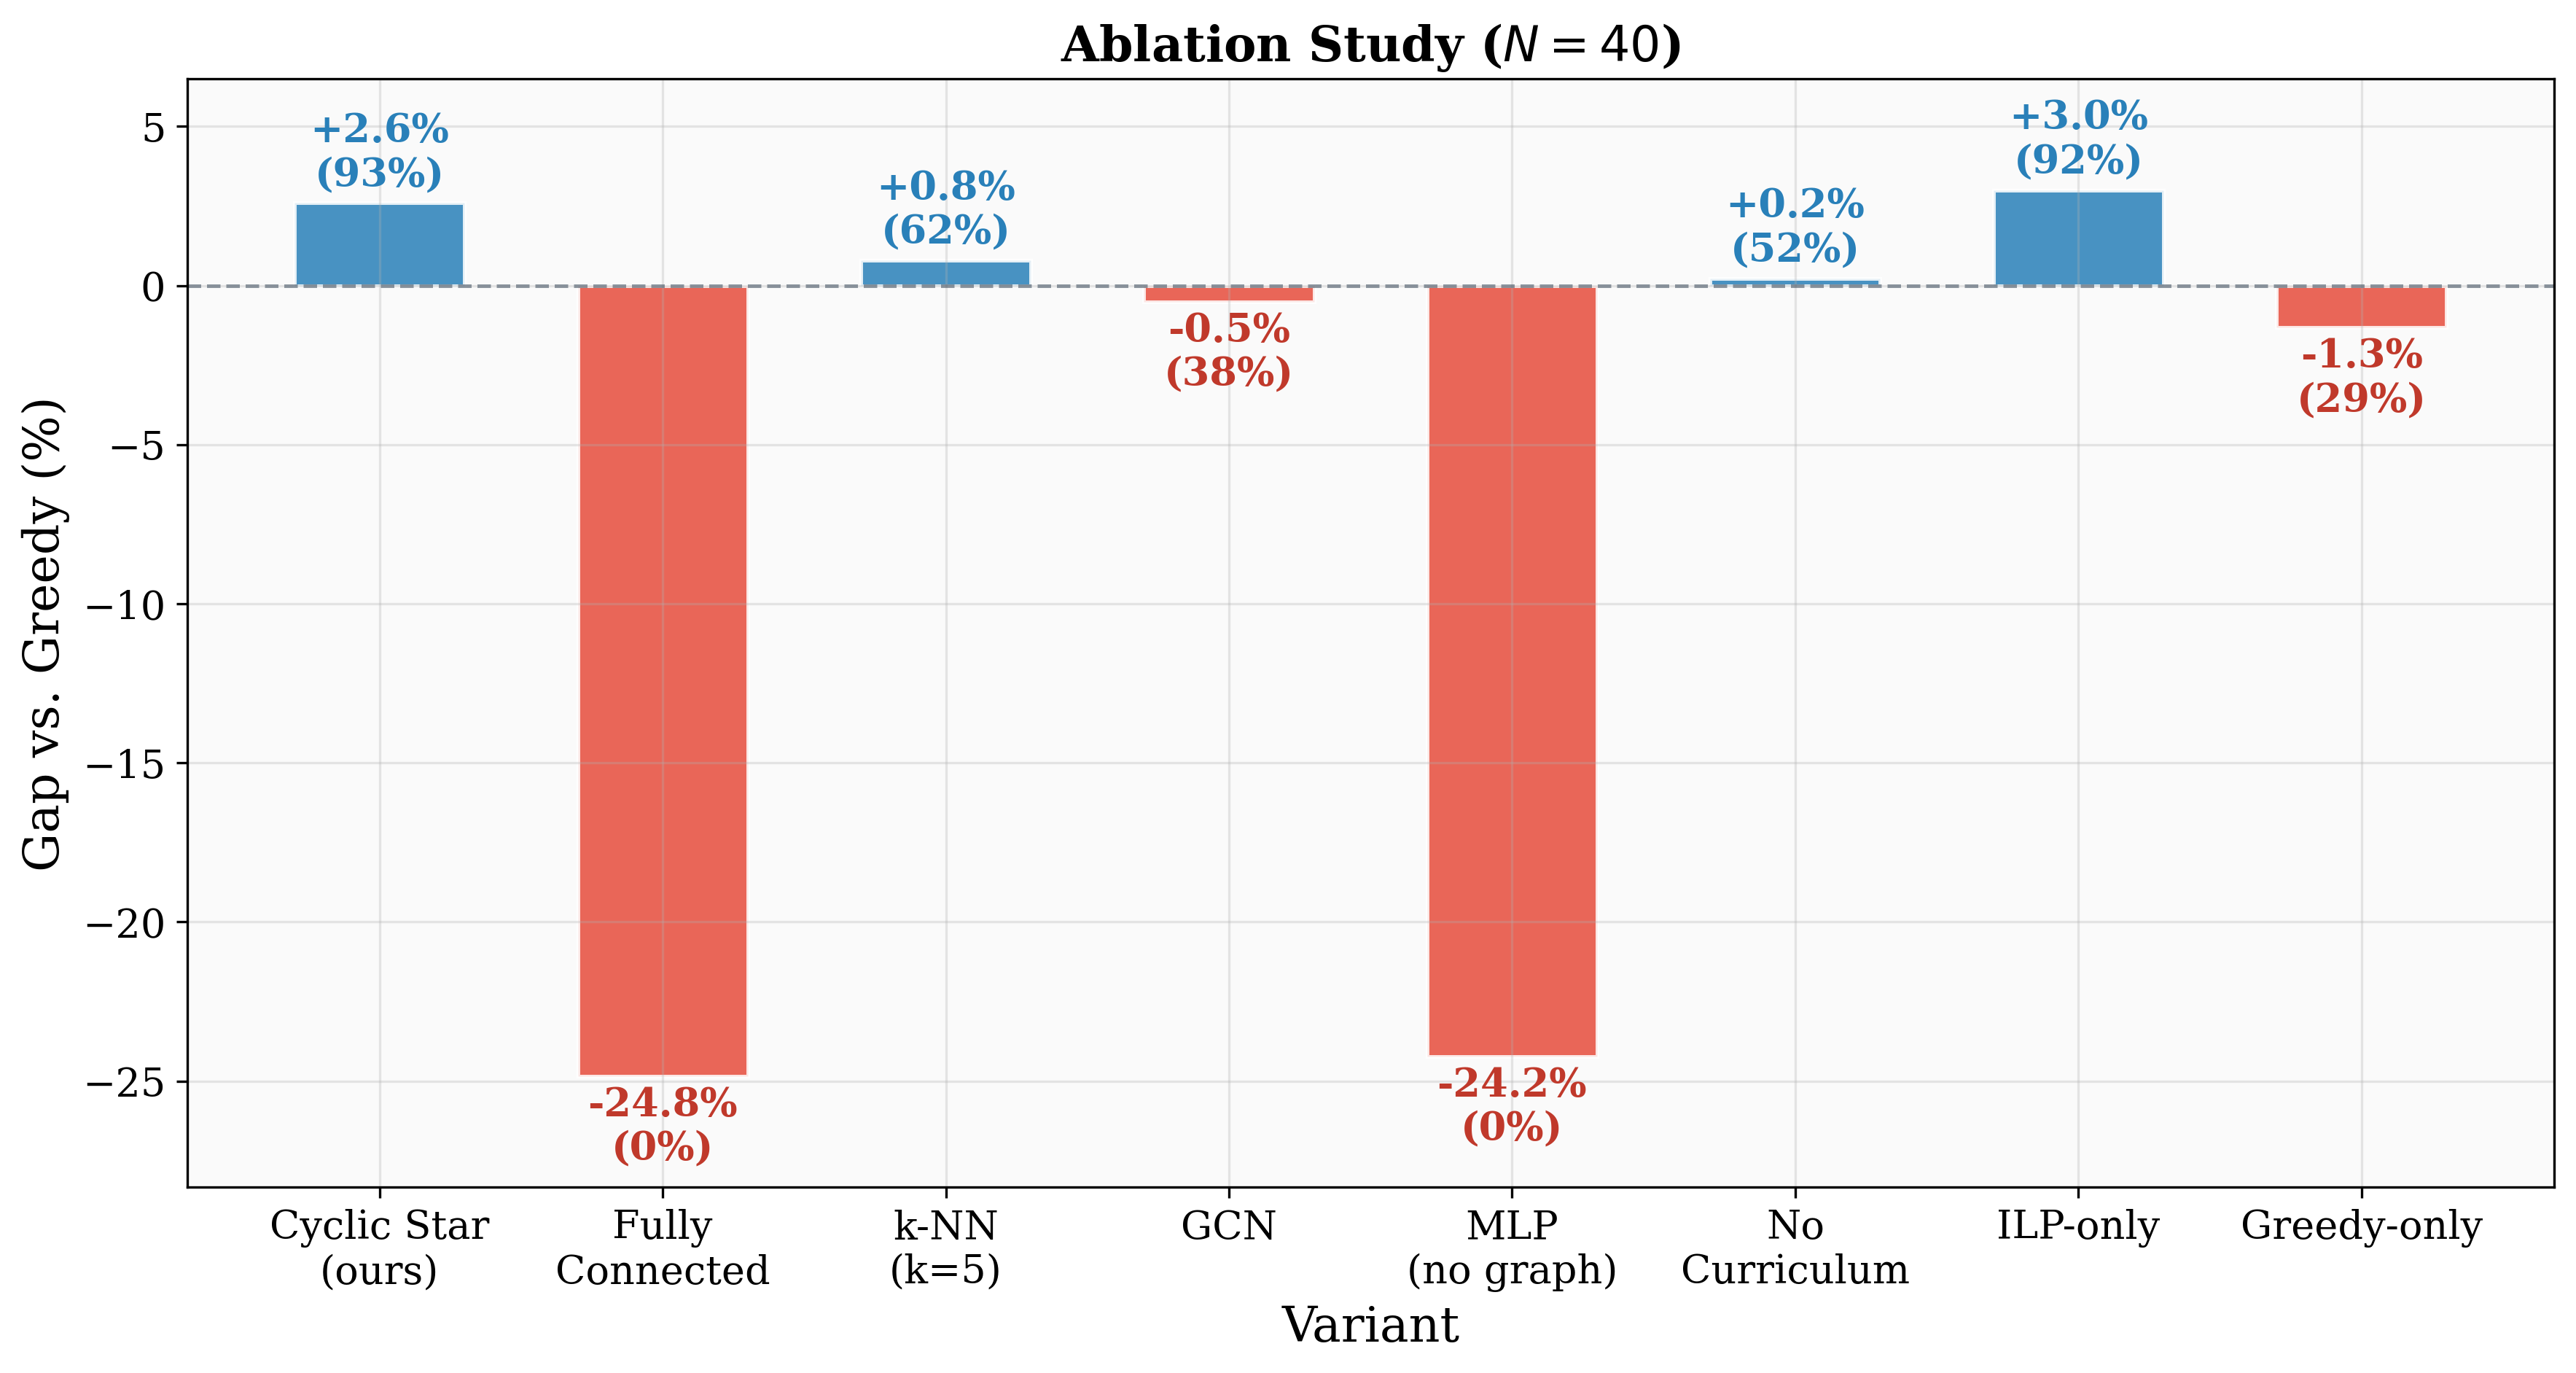
\includegraphics[width=0.9\linewidth]{figures/paper/fig_ablations.png}
\caption{Ablation results ($N{=}40$). Bars show gap vs.\ greedy (\%) with win-rates annotated. Fully connected graphs and MLP (no graph) fail catastrophically; greedy-only supervision cannot beat greedy. The proposed configuration (cyclic star + GAT + ILP supervision) achieves consistently positive improvement.}
\label{fig:ablations}
\end{figure}

\subsection{Comparison with Improvement Heuristics}

At small scales ($N{=}10$), classical improvement heuristics (2-opt, SA) are expected to achieve costs comparable to the GNN since the search space is small enough for iterative refinement. At $N{=}40$, the GNN's single forward pass offers a potential runtime advantage over SA's iterative cooling schedule, though direct cost and timing comparisons are pending.

\subsection{Limitations}

We acknowledge several gaps. Generalisation to out-of-distribution scenarios (e.g., training on $N{=}20$, testing on $N{=}40$; training on corner bins, testing on random bin placements) has not been evaluated. The $N{=}200$ evaluation (Table~\ref{tab:results_200obj}) uses 100 scenarios but lacks paired significance testing. The imitation learning framework is subject to covariate shift \cite{ross2011dagger}; DAgger-style online data collection or RL fine-tuning could address this. The cost model uses Euclidean distance; kinematic or dynamic robot models would improve applicability to specific manipulator platforms.

%========================================================================
\section{Conclusion}\label{sec:conclusion}
%========================================================================

We have presented a method for distilling the decision quality of an exact ILP solver into a lightweight GNN policy for robotic pick-and-place sequencing. The key architectural enabler is the cyclic star graph that explicitly represents the causal structure of pick-and-place actions: robot, object, and bin nodes connected by directed edges encoding the full pick-place-feedback cycle. Type information is encoded in node features and processed by a standard GAT. This structural representation captures information that flat sequence-to-sequence NCO architectures fundamentally discard.

Trained via curriculum-based imitation learning on ILP-optimal prefixes with greedy fallback, the policy reaches 1.81\% mean ILP gap at $N{=}10$ (with exact matches on a subset of instances), 98\% win-rate vs.\ greedy at $N{=}40$ (98/100 scenarios, $p < 10^{-31}$), and scales to $N{=}200$ where exact ILP is entirely intractable. The distillation framework extends near-optimal sequencing beyond the computational reach of the solver itself.

Future work includes: DAgger or RL fine-tuning to address covariate shift, extension to online conveyor-belt settings with temporal constraints, kinematic cost models for specific manipulator platforms \cite{han2019pap} with obstacle-aware edge costs derived from motion planners such as dynamic PRM reshaping \cite{ojha2025obstacle}, cross-distribution generalisation experiments, and validation on physical robotic sorting systems.

\section*{Acknowledgment}
% Add acknowledgments here.

\appendices
\section{Node Feature Vector Layout}\label{app:features}

Each node feature has dimension $F = 4 + M + 1 = 9$ (with $M{=}4$ bins). We use a unified layout:
\begin{equation}
x_i = [p^{(\text{self})}_x, p^{(\text{self})}_y,\; p^{(\text{ref})}_x, p^{(\text{ref})}_y,\; \text{onehot}(\text{type})_{1:M},\; m].
\end{equation}

\textbf{Object nodes:} $p^{(\text{self})}$ is the object position (normalised by $W$), $p^{(\text{ref})}$ is the target bin position determined by the object type, $\text{onehot}(\text{type})$ encodes the assigned bin, and $m \in \{0,1\}$ is the availability mask. The reference position encodes the placement-leg destination directly, enabling the GNN to reason about full cycle cost without multi-hop message passing to discover bin locations.

\textbf{Robot node:} Normalised position in $p^{(\text{self})}$; remaining dimensions zero-padded.

\textbf{Bin nodes:} Bin position in both $p^{(\text{self})}$ and $p^{(\text{ref})}$; identity basis for $\text{onehot}(\text{type})$; $m{=}0$.

%========================================================================
\begin{thebibliography}{00}

\bibitem{vinyals2015pointer} O.~Vinyals, M.~Fortunato, and N.~Jaitly, ``Pointer Networks,'' in \emph{Advances in Neural Information Processing Systems (NeurIPS)}, vol.~28, 2015.

\bibitem{kool2019attention} W.~Kool, H.~Van Hoof, and M.~Welling, ``Attention, learn to solve routing problems!'' in \emph{International Conference on Learning Representations (ICLR)}, 2019.

\bibitem{kwon2020pomo} Y.~D.~Kwon, J.~Choo, B.~Kim, I.~Yoon, Y.~Gwon, and S.~Min, ``POMO: Policy optimization with multiple optima for reinforcement learning,'' in \emph{NeurIPS}, vol.~33, pp.~21188--21198, 2020.

\bibitem{costa2020learning2opt} P.~R.~d~O~Costa, J.~Rhuggenaath, Y.~Zhang, and A.~Akcay, ``Learning 2-opt heuristics for the traveling salesman problem via deep reinforcement learning,'' in \emph{ACML}, PMLR, pp.~465--480, 2020.

\bibitem{kim2022symnco} M.~Kim, J.~Park, and J.~Park, ``Sym-NCO: Leveraging symmetricity for neural combinatorial optimization,'' in \emph{NeurIPS}, vol.~35, pp.~1936--1949, 2022.

\bibitem{cappart2023gnnco} Q.~Cappart, D.~Ch\'{e}telat, E.~B.~Khalil, A.~Lodi, C.~Morris, and P.~Veli\v{c}kovi\'{c}, ``Combinatorial optimization and reasoning with graph neural networks,'' \emph{JMLR}, vol.~24, no.~130, pp.~1--61, 2023.

\bibitem{perera2023gpn} J.~Perera, S.-H.~Liu, M.~Mernik, M.~\v{C}repin\v{s}ek, and M.~Ravber, ``A graph pointer network-based multi-objective deep reinforcement learning algorithm for solving the traveling salesman problem,'' \emph{Mathematics}, vol.~11, no.~2, p.~437, 2023.

\bibitem{xiong2025ropt} Z.~Xiong, Y.~Wang, Y.~Tian, L.~Liu, and S.~Zhu, ``RoPT: Route-planning model with transformer,'' \emph{Applied Sciences}, vol.~15, no.~9, p.~4914, 2025.

\bibitem{chung2025ncosurvey} K.~T.~Chung, C.~K.~M.~Lee, and Y.~P.~Tsang, ``Neural combinatorial optimization with reinforcement learning in industrial engineering: a survey,'' \emph{Artificial Intelligence Review}, vol.~58, p.~130, 2025.

\bibitem{han2019pap} S.~D.~Han, S.~W.~Feng, and J.~Yu, ``Toward fast and optimal robotic pick-and-place on a moving conveyor,'' \emph{IEEE Robot.\ Autom.\ Lett.}, vol.~5, no.~2, pp.~446--453, Apr.\ 2020.

\bibitem{kiyokawa2024challenges} T.~Kiyokawa, J.~Takamatsu, and S.~Koyanaka, ``Challenges for future robotic sorters of mixed industrial waste: A survey,'' \emph{IEEE Trans.\ Autom.\ Sci.\ Eng.}, vol.~21, pp.~1023--1040, 2024.

\bibitem{chalasani1996} P.~Chalasani, R.~Motwani, and A.~Rao, ``Algorithms for robot grasp and delivery,'' in \emph{2nd WAFR}, 1996.

\bibitem{rosenkrantz1977} D.~J.~Rosenkrantz, R.~E.~Stearns, and P.~M.~Lewis, ``An analysis of several heuristics for the traveling salesman problem,'' \emph{SIAM J.\ Comput.}, vol.~6, no.~3, pp.~563--581, 1977.

\bibitem{cheng2024drl} B.~Cheng, T.~Xie, L.~Wang, Q.~Tan, and X.~Cao, ``Deep reinforcement learning driven cost minimization for batch order scheduling in robotic mobile fulfillment systems,'' \emph{Expert Systems with Applications}, vol.~255, 2024.

\bibitem{ross2011dagger} S.~Ross, G.~Gordon, and D.~Bagnell, ``A reduction of imitation learning and structured prediction to no-regret online learning,'' in \emph{AISTATS}, PMLR~15, pp.~627--635, 2011.

\bibitem{loshchilov2019adamw} I.~Loshchilov and F.~Hutter, ``Decoupled weight decay regularization,'' in \emph{ICLR}, 2019.

\bibitem{dantzig1954} G.~Dantzig, D.~R.~Fulkerson, and S.~M.~Johnson, ``Solution of a large-scale traveling-salesman problem,'' \emph{J.\ Oper.\ Res.\ Soc.\ Am.}, vol.~2, no.~4, pp.~393--410, 1954.

\bibitem{gundupalli2021sequence} S.~P.~Gundupalli, R.~Shukla, R.~Gupta, S.~Hait, and A.~Thakur, ``Optimal sequence planning for robotic sorting of recyclables from source-segregated municipal solid waste,'' \emph{J.\ Comput.\ Inf.\ Sci.\ Eng.}, vol.~21, no.~1, p.~014502, 2021.

\bibitem{ojha2025obstacle} P.~Ojha and A.~Thakur, ``Dynamic obstacle avoidance using path reshaping on probabilistic roadmaps for high-degree-of-freedom robots,'' \emph{IEEE Trans.\ Artif.\ Intell.}, vol.~7, no.~2, 2026.

\end{thebibliography}

\end{document}
